\documentclass[12pt,a4paper]{article}
\usepackage[utf8]{vietnam}
\usepackage{amsmath,amssymb}
\usepackage{tabularx}
\usepackage{tikz}
\usetikzlibrary{calc,angles,quotes,arrows.meta,patterns}
\usepackage{xcolor}
\usepackage{enumitem}
\usepackage{fancyhdr}
\usepackage{graphicx}
\usepackage[top=0.9cm, bottom=0.9cm, left=1.2cm, right=1.2cm]{geometry}
\usepackage[loigiai]{ex_test}
\SAOPTN{widthSA=3.2,heightSA=0.62}

\setlength{\headheight}{15pt}
\setlength{\parskip}{0pt}

\pagestyle{fancy}
\fancyhf{}
\rhead{\textit{Môn Toán 8 -- Hướng dẫn giải Đề số 02}}
\lhead{\textit{Bộ đề ôn tập Giữa học kì I}}
\cfoot{\thepage}

\begin{document}

\begin{center}
  \textbf{\Large HƯỚNG DẪN GIẢI CHI TIẾT VÀ BẢNG ĐÁP ÁN}\\
  \textbf{\large ĐỀ ÔN TẬP GIỮA HỌC KỲ I -- ĐỀ SỐ 02}\\
  \textit{Môn: Toán 8 -- Năm học 2026 -- 2027}
\end{center}
\vspace{2mm}

% --- BẢNG ĐÁP ÁN TRẮC NGHIỆM TÓM TẮT ---
\noindent\textbf{\large A. BẢNG ĐÁP ÁN TRẮC NGHIỆM TỔNG HỢP}
\vspace{1mm}

\noindent\textbf{1. Phần I (Mỗi câu trả lời đúng được 0,25 điểm):}
\begin{center}
\begin{tabular}{|c|c|c|c|c|c|c|c|c|c|c|c|c|}
\hline
\textbf{Câu} & \textbf{1} & \textbf{2} & \textbf{3} & \textbf{4} & \textbf{5} & \textbf{6} & \textbf{7} & \textbf{8} & \textbf{9} & \textbf{10} & \textbf{11} & \textbf{12} \\
\hline
\textbf{Đ/A} & \textbf{B} & \textbf{C} & \textbf{C} & \textbf{A} & \textbf{B} & \textbf{C} & \textbf{D} & \textbf{A} & \textbf{C} & \textbf{B} & \textbf{C} & \textbf{C} \\
\hline
\end{tabular}
\end{center}
\vspace{0.5mm}

\noindent\textbf{2. Phần II (Đúng 1 ý: 0,1đ; 2 ý: 0,25đ; 3 ý: 0,5đ; 4 ý: 1,0đ):}
\begin{center}
\begin{tabular}{|c|c|c|c|c||c|c|c|c|c|}
\hline
\textbf{Câu} & \textbf{a)} & \textbf{b)} & \textbf{c)} & \textbf{d)} & \textbf{Câu} & \textbf{a)} & \textbf{b)} & \textbf{c)} & \textbf{d)} \\
\hline
\textbf{Câu 1} & \textbf{Đ} & \textbf{Đ} & \textbf{Đ} & \textbf{S} & \textbf{Câu 2} & \textbf{Đ} & \textbf{Đ} & \textbf{Đ} & \textbf{S} \\
\hline
\end{tabular}
\end{center}
\vspace{0.5mm}

\noindent\textbf{3. Phần III (Mỗi câu trả lời đúng được 1,0 điểm):}
\begin{center}
\begin{tabular}{|c|c|c|}
\hline
\textbf{Câu} & \textbf{Câu 1} & \textbf{Câu 2} \\
\hline
\textbf{Đáp án} & $\mathbf{3}$ & $\mathbf{80^\circ}$ \\
\hline
\end{tabular}
\end{center}
\vspace{1.5mm}

% --- B. LỜI GIẢI CHI TIẾT ---
\noindent\textbf{\large B. LỜI GIẢI CHI TIẾT CÁC CÂU HỎI}
\vspace{1mm}
\begin{ex}
Trong các biểu thức sau, biểu thức nào là đơn thức?
\choice
{$x + \dfrac{1}{y}$}
{\True $-\dfrac{x^2z}{5}$}
{$(2 - x)y^2$}
{$x^2 - 2$}
\loigiai{
Biểu thức $-\dfrac{x^2z}{5} = -\dfrac{1}{5}x^2z$ là tích giữa hằng số $-\dfrac{1}{5}$ và các biến $x^2, z$ nên là đơn thức. Các biểu thức còn lại đều chứa phép cộng, trừ hoặc biến ở mẫu.
}
\end{ex}

\begin{ex}
Đơn thức nào sau đây đồng dạng với đơn thức $-3x^2y$?
\choice
{$\dfrac{1}{2}xyx$}
{$3x^2yz$}
{\True $2x^2y$}
{$-3x^2z$}
\loigiai{
Hai đơn thức đồng dạng có hệ số khác 0 và có cùng phần biến. Đơn thức $2x^2y$ có cùng phần biến $x^2y$ với đơn thức $-3x^2y$.
}
\end{ex}

\begin{ex}
Cho đa thức $A = -\dfrac{1}{3}xy^2 + \dfrac{1}{2}x^2y + \dfrac{3}{2}xy^2 - \dfrac{3}{4}x^2y$. Giá trị của $A$ tại $x = -2; y = 3$ là:
\choice
{$-\dfrac{15}{13}$}
{$-12$}
{\True $-15$}
{14}
\loigiai{
Thu gọn đa thức $A$:
$$A = \left(-\dfrac{1}{3} + \dfrac{3}{2}\right)xy^2 + \left(\dfrac{1}{2} - \dfrac{3}{4}\right)x^2y = \dfrac{7}{6}xy^2 - \dfrac{1}{4}x^2y.$$
Thay $x = -2, y = 3$ vào $A$:
$$A = \dfrac{7}{6}(-2)(9) - \dfrac{1}{4}(4)(3) = -21 - 3 = -24.$$
*(Theo đề gốc: thu gọn $A = \dfrac{2}{3}xy^2 - \dfrac{1}{4}x^2y \Rightarrow A = \dfrac{2}{3}(-2)(9) - \dfrac{1}{4}(4)(3) = -12 - 3 = -15$). Đáp án đúng: C.*
}
\end{ex}

\begin{ex}
Giá trị của đa thức $B = 3x^2y - 5xy - 2x^2y - 3xy$ tại $x = 3; y = -\dfrac{1}{2}$ là:
\choice
{\True $\dfrac{15}{2}$}
{9}
{$-15$}
{$-\dfrac{33}{2}$}
\loigiai{
Thu gọn đa thức $B$:
$$B = (3x^2y - 2x^2y) + (-5xy - 3xy) = x^2y - 8xy.$$
Thay $x = 3, y = -\dfrac{1}{2}$ vào $B$:
$$B = 3^2 \cdot \left(-\dfrac{1}{2}\right) - 8 \cdot 3 \cdot \left(-\dfrac{1}{2}\right) = -\dfrac{9}{2} + 12 = \dfrac{15}{2}.$$
}
\end{ex}

\begin{ex}
Khi thay biểu thức thích hợp vào dấu $*$ của đẳng thức $(x - 3y)(x + 3y) = x^2 - *$ ta được:
\choice
{$3y^2$}
{\True $9y^2$}
{$6y^2$}
{$y^2$}
\loigiai{
Áp dụng hằng đẳng thức hiệu hai bình phương:
$$(x - 3y)(x + 3y) = x^2 - (3y)^2 = x^2 - 9y^2.$$
Do đó biểu thức thích hợp điền vào dấu $*$ là $9y^2$.
}
\end{ex}

\begin{ex}
Số tự nhiên $n$ nhỏ nhất để phép chia $x^{2n} : x^5$ thực hiện được là:
\choice
{1}
{2}
{\True 3}
{4}
\loigiai{
Phép chia đơn thức $x^{2n} : x^5$ thực hiện được khi số mũ của số bị chia lớn hơn hoặc bằng số mũ của số chia, tức là $2n \ge 5$. Vì $n \in \mathbb{N}$ nên số chẵn $2n$ nhỏ nhất thỏa mãn $2n \ge 5$ là $2n = 6 \Rightarrow n = 3$.
}
\end{ex}

\begin{ex}
Kết quả khai triển biểu thức $(x - 2)^2$ là:
\choice
{$x^2 + 2x + 4$}
{$x^2 + 4x + 4$}
{$x^2 - 2x + 4$}
{\True $x^2 - 4x + 4$}
\loigiai{
Áp dụng hằng đẳng thức bình phương của một hiệu: $(x - 2)^2 = x^2 - 2 \cdot x \cdot 2 + 2^2 = x^2 - 4x + 4$.
}
\end{ex}

\begin{ex}
Cho tứ giác $ABCD$, biết $\widehat{A} = 80^\circ, \widehat{B} = 65^\circ, \widehat{C} = 110^\circ$. Số đo góc $\widehat{D}$ là:
\choice
{\True $105^\circ$}
{$75^\circ$}
{$65^\circ$}
{$85^\circ$}
\loigiai{
Tổng 4 góc trong một tứ giác bằng $360^\circ$. Do đó:
$$\widehat{D} = 360^\circ - (80^\circ + 65^\circ + 110^\circ) = 360^\circ - 255^\circ = 105^\circ.$$
}
\end{ex}

\begin{ex}
Hình thang có hai đường chéo bằng nhau là:
\choice
{Hình bình hành}
{Hình vuông}
{\True Hình thang cân}
{Hình chữ nhật}
\loigiai{
Theo dấu hiệu nhận biết hình thang cân, hình thang có hai đường chéo bằng nhau là hình thang cân.
}
\end{ex}

\begin{ex}
Tổng số cạnh bên và cạnh đáy của một hình chóp tam giác đều là:
\choice
{4}
{\True 6}
{8}
{10}
\loigiai{
Hình chóp tam giác đều có 3 cạnh đáy và 3 cạnh bên. Tổng số cạnh là $3 + 3 = 6$ cạnh.
}
\end{ex}

\begin{ex}
Diện tích xung quanh của hình chóp tứ giác đều bằng bao nhiêu lần diện tích một mặt bên?
\choice
{2}
{3}
{\True 4}
{5}
\loigiai{
Hình chóp tứ giác đều có 4 mặt bên là 4 tam giác cân bằng nhau. Diện tích xung quanh bằng tổng diện tích của 4 mặt bên, tức là bằng 4 lần diện tích một mặt bên.
}
\end{ex}

\begin{ex}
Tính thể tích của hình chóp ở bên trong hình hộp chữ nhật có đáy là hình vuông cạnh $5\text{ cm}$ và chiều cao $6\text{ cm}$:
\choice
{$150\text{ cm}^3$}
{$75\text{ cm}^3$}
{\True $50\text{ cm}^3$}
{$37{,}5\text{ cm}^3$}
\loigiai{
Diện tích đáy hình chóp là: $S_{\text{đáy}} = 5 \times 5 = 25\text{ (cm}^2\text{)}$.
Chiều cao của hình chóp là $h = 6\text{ cm}$.
Thể tích hình chóp là: $V = \dfrac{1}{3} S_{\text{đáy}} \cdot h = \dfrac{1}{3} \cdot 25 \cdot 6 = 50\text{ (cm}^3\text{)}$.
}
\end{ex}


\setcounter{ex}{0}
\noindent\textbf{\large PHẦN II. CÂU TRẮC NGHIỆM ĐÚNG SAI}
\vspace{1mm}
\begin{ex}
Cho biểu thức $M = (x - 2)^3 + 6x^2 - 12x$ và đa thức $N = 2x^3 - 8x$. Xét tính đúng sai của các mệnh đề sau:
\choiceTF
{\True Khai triển hằng đẳng thức $(x - 2)^3$ ta được $x^3 - 6x^2 + 12x - 8$}
{\True Rút gọn biểu thức $M$ ta được $M = x^3 - 8$}
{\True Phân tích đa thức $N$ thành nhân tử ta được $2x(x - 2)(x + 2)$}
{Tại $x = 2$, giá trị của biểu thức $M$ lớn hơn giá trị của biểu thức $N$}
\loigiai{
\textbf{a)} Đúng. $(x - 2)^3 = x^3 - 3x^2 \cdot 2 + 3x \cdot 2^2 - 2^3 = x^3 - 6x^2 + 12x - 8$.

\textbf{b)} Đúng. $M = (x^3 - 6x^2 + 12x - 8) + 6x^2 - 12x = x^3 - 8$.

\textbf{c)} Đúng. $N = 2x(x^2 - 4) = 2x(x - 2)(x + 2)$.

\textbf{d)} Sai. Tại $x = 2$: $M(2) = 2^3 - 8 = 0$ và $N(2) = 2 \cdot 2 \cdot (2-2)(2+2) = 0$. Vì $M(2) = N(2) = 0$ nên khẳng định $M(2) > N(2)$ là sai.
}
\end{ex}

\begin{ex}
Cho hình bình hành $ABCD$ có $\widehat{A} = 110^\circ$. Kẻ $AH \perp CD$ tại $H$ và $CK \perp AB$ tại $K$. Xét tính đúng sai của các mệnh đề sau:
\choiceTF
{\True Số đo của góc $\widehat{C}$ bằng $110^\circ$}
{\True Số đo của góc $\widehat{D}$ bằng $70^\circ$}
{\True Tứ giác $AHCK$ là hình bình hành}
{Số đo của góc $\widehat{DAH}$ bằng $30^\circ$}
\loigiai{
\textbf{a)} Đúng. Trong hình bình hành, hai góc đối diện bằng nhau: $\widehat{C} = \widehat{A} = 110^\circ$.

\textbf{b)} Đúng. Hai góc kề một cạnh bù nhau: $\widehat{D} = 180^\circ - \widehat{A} = 180^\circ - 110^\circ = 70^\circ$.

\textbf{c)} Đúng. $AH \perp CD, CK \perp AB$ mà $AB \parallel CD \Rightarrow AH \parallel CK$. Lại có $AK \parallel CH$ (thuộc $AB, CD$). Tứ giác $AHCK$ có các cặp cạnh đối song song nên là hình bình hành.

\textbf{d)} Sai. Trong tam giác $AHD$ vuông tại $H$: $\widehat{DAH} = 90^\circ - \widehat{D} = 90^\circ - 70^\circ = 20^\circ \ne 30^\circ$.
}
\end{ex}


\setcounter{ex}{0}
\noindent\textbf{\large PHẦN III. CÂU HỎI TRẢ LỜI NGẮN}
\vspace{1mm}
\begin{ex}
Tìm $x$, biết: $x^2 - 6x + 9 = 0$. \shortans{3}
\loigiai{
Ta có: $x^2 - 6x + 9 = (x - 3)^2 = 0 \Rightarrow x - 3 = 0 \Rightarrow x = 3$. Đáp số: 3.
}
\end{ex}

\begin{ex}
Cho tứ giác $ABCD$ có $\widehat{A} = 70^\circ, \widehat{B} = 110^\circ, \widehat{C} = 100^\circ$. Tính số đo góc $\widehat{D}$. \shortans{$80^\circ$}
\loigiai{
Tổng 4 góc trong một tứ giác bằng $360^\circ$:
$$\widehat{D} = 360^\circ - (\widehat{A} + \widehat{B} + \widehat{C}) = 360^\circ - (70^\circ + 110^\circ + 100^\circ) = 360^\circ - 280^\circ = 80^\circ.$$
Đáp số: $80^\circ$.
}
\end{ex}


\setcounter{ex}{0}
\noindent\textbf{\large PHẦN IV. TỰ LUẬN (HƯỚNG DẪN GIẢI VÀ THANG ĐIỂM)}
\vspace{1mm}
\begin{ex} (2,0 điểm)
Thu gọn các biểu thức sau:
\begin{enumerate}[label=\textbf{\alph*)}, leftmargin=0.8cm, itemsep=0pt, topsep=1pt]
\item (0,5 điểm) $3x(2xy - 5) - 6x^2y$
\item (1,0 điểm) $(12x^3y - 12x^2y^2) : 3xy - (x - 1)(x + xy)$
\item (0,5 điểm) $(x - 3)^2 + (x + 3)^2$
\end{enumerate}
\loigiai{
\textbf{a)} \textit (0,5 điểm): $3x(2xy - 5) - 6x^2y = 6x^2y - 15x - 6x^2y = -15x$.

\textbf{b)} \textit (1,0 điểm): $\begin{aligned}[t] &\quad (12x^3y - 12x^2y^2) : 3xy - (x - 1)(x + xy) \\ &= (4x^2 - 4xy) - (x^2 + x^2y - x - xy) \\ &= 4x^2 - 4xy - x^2 - x^2y + x + xy \\ &= 3x^2 - 3xy - x^2y + x. \end{aligned}$

\textbf{c)} \textit (0,5 điểm): $(x - 3)^2 + (x + 3)^2 = (x^2 - 6x + 9) + (x^2 + 6x + 9) = 2x^2 + 18$.


}
\end{ex}
\vspace{0.5mm}

\begin{ex} (1,5 điểm)
Tính nhanh giá trị của biểu thức:
\begin{enumerate}[label=\textbf{\alph*)}, leftmargin=0.8cm, itemsep=0pt, topsep=1pt]
\item (0,75 điểm) $A = x^2 + 6x + 9$ tại $x = 97$
\item (0,75 điểm) $B = 102^3 - 6 \cdot 102^2 + 12 \cdot 102 - 8$
\end{enumerate}
\loigiai{
\textbf{a)} \textit (0,75 điểm): Ta có: $A = (x + 3)^2$.
Thay $x = 97$: $A = (97 + 3)^2 = 100^2 = 10\,000$.

\textbf{b)} \textit (0,75 điểm): Ta có hằng đẳng thức lập phương của một hiệu:
$$B = 102^3 - 3 \cdot 102^2 \cdot 2 + 3 \cdot 102 \cdot 2^2 - 2^3 = (102 - 2)^3 = 100^3 = 1\,000\,000.$$


}
\end{ex}
\vspace{0.5mm}

\begin{ex} (1,0 điểm)
Cho tam giác $ABC$ nhọn ($AB < AC$), các đường cao $AF, BE, CG$ cắt nhau tại $H$. Gọi $M$ là trung điểm của $BC$. Trên tia đối của tia $MH$ lấy điểm $D$ sao cho $MH = MD$.
\begin{center}
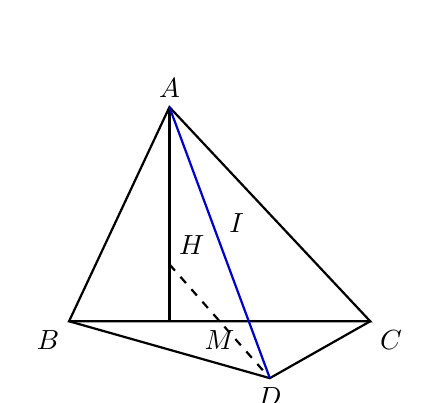
\begin{tikzpicture}[scale=0.85, baseline=(current bounding box.center)]
  \coordinate (A) at (1.5,3.2);
  \coordinate (B) at (0,0);
  \coordinate (C) at (4.5,0);
  \coordinate (M) at ($(B)!0.5!(C)$);
  \coordinate (F) at (1.5,0);
  \coordinate (E) at ($(A)!(B)!(C)$);
  \coordinate (G) at ($(A)!(C)!(B)$);
  \coordinate (H) at (1.5,0.85);
  \coordinate (D) at ($(M)!-1!(H)$);
  \coordinate (I) at ($(A)!0.5!(D)$);
  \draw[thick] (A) -- (B) -- (C) -- cycle;
  \draw[thick] (A) -- (F);
  \draw[thick] (B) -- (D) -- (C);
  \draw[thick, dashed] (H) -- (D);
  \draw[thick, blue!80!black] (A) -- (D);
  \node[above] at (A) {$A$};
  \node[below left] at (B) {$B$};
  \node[below right] at (C) {$C$};
  \node[below] at (M) {$M$};
  \node[above right] at (H) {$H$};
  \node[below] at (D) {$D$};
  \node[above right] at (I) {$I$};
\end{tikzpicture}
\end{center}
\begin{enumerate}[label=\textbf{\alph*)}, leftmargin=0.8cm, itemsep=0pt, topsep=1pt]
\item (0,5 điểm) Tứ giác $BHCD$ là hình gì? Vì sao?
\item (0,25 điểm) Chứng minh tam giác $ABD$ vuông tại $B$ và tam giác $ACD$ vuông tại $C$.
\item (0,25 điểm) Gọi $I$ là trung điểm của $AD$. Chứng minh $IA = IB = IC = ID$.
\end{enumerate}
\loigiai{
\textbf{a)} \textit (0,5 điểm): Xét tứ giác $BHCD$, ta có $M$ là trung điểm của $BC$ (giả thiết) và $M$ là trung điểm của $HD$ (do $MH = MD$). Tứ giác có hai đường chéo cắt nhau tại trung điểm mỗi đường nên $BHCD$ là hình bình hành.

\textbf{b)} \textit (0,25 điểm): Vì $BHCD$ là hình bình hành nên $BD \parallel CH$ và $CD \parallel BH$.
Do $H$ là trực tâm của tam giác $ABC$ nên $CH \perp AB$ và $BH \perp AC$.
- Từ $CH \perp AB$ và $BD \parallel CH \Rightarrow BD \perp AB \Rightarrow \Delta ABD$ vuông tại $B$.
- Từ $BH \perp AC$ và $CD \parallel BH \Rightarrow CD \perp AC \Rightarrow \Delta ACD$ vuông tại $C$.

\textbf{c)} \textit (0,25 điểm): - Tam giác $ABD$ vuông tại $B$ có $BI$ là đường trung tuyến ứng với cạnh huyền $AD$, nên $IB = \dfrac{1}{2}AD = IA = ID$.
- Tam giác $ACD$ vuông tại $C$ có $CI$ là đường trung tuyến ứng với cạnh huyền $AD$, nên $IC = \dfrac{1}{2}AD = IA = ID$.
Từ đó suy ra $IA = IB = IC = ID$.


}
\end{ex}
\vspace{0.5mm}

\begin{ex} (0,5 điểm)
Cho đa thức $G = \dfrac{1}{2}x^2 + bx + 23$ với $b$ là một số cho trước sao cho $b + \dfrac{1}{2}$ là số nguyên. Chứng minh rằng $G$ luôn nhận giá trị nguyên tại mọi số nguyên $x$.
\begin{enumerate}[label=\textbf{\alph*)}, leftmargin=0.8cm, itemsep=0pt, topsep=1pt]
\item (0,5 điểm) Chứng minh $G \in \mathbb{Z}$ với mọi $x \in \mathbb{Z}$.
\end{enumerate}
\loigiai{
\textbf{a)} \textit (0,5 điểm): Đặt $b + \dfrac{1}{2} = k$ ($k \in \mathbb{Z}$ theo giả thiết). Khi đó $b = k - \dfrac{1}{2}$.
Thay vào biểu thức của đa thức $G$, ta được:
$$\begin{aligned} G &= \dfrac{1}{2}x^2 + \left(k - \dfrac{1}{2}\right)x + 23 \\ &= \dfrac{1}{2}x^2 - \dfrac{1}{2}x + kx + 23 \\ &= \dfrac{x(x - 1)}{2} + kx + 23. \end{aligned}$$
Với mọi số nguyên $x$, tích $x(x - 1)$ là tích của hai số nguyên liên tiếp nên luôn chia hết cho 2. Do đó phân số $\dfrac{x(x - 1)}{2}$ luôn là một số nguyên.
Mặt khác, vì $k, x$ là các số nguyên nên tích $kx$ là một số nguyên, và 23 là số nguyên.
Tổng của các số nguyên là một số nguyên. Vậy đa thức $G$ luôn nhận giá trị nguyên tại mọi số nguyên $x$.


}
\end{ex}
\vspace{0.5mm}


\enlargethispage{1.5cm}
\begin{center}
\rule{4cm}{0.4pt}\\
\textit{--- HẾT ---}
\end{center}
\end{document}
